\chapter{Exam Questions}
\section{Mathematics}
\begin{Exercise}
Say we wish to rotate an arbitrary point $(x,y,z)$ over an angle $\theta$
around the point $(2,1,3)$ in the plane XZ.
Give two ways to compute this.
\begin{solution}
\begin{itemize}
  \item Using quaternions. Rotated point has coordinates $(x' + 2, y' + 1, z' + 3)$:
        \[
          \begin{array}{rcl}
            q & = & (x - 2) i+(y - 1) j+(z - 3) k \\ \\
            r & = & \displaystyle \cos\left(\frac\theta2\right) +
                    \sin\left(\frac\theta2\right) j \\ \\
            \conj{r} & = & \displaystyle \cos\left(\frac\theta2\right) -
                           \sin\left(\frac\theta2\right) j \\ \\
            x'i+y'j+z'k & = & r \cdot q \cdot \conj{r} \\
          \end{array}
        \]
  \item Using matrices
        \[
          \left[
            \begin{array}{c}
              x' \\
              y' \\
              z' \\
              1
            \end{array}
          \right]
          =
          \left[
            \begin{array}{cccc}
              1 & 0 & 0 & 2 \\
              0 & 1 & 0 & 1 \\
              0 & 0 & 1 & 3 \\
              0 & 0 & 0 & 1 \\
            \end{array}
          \right]
          \cdot
          \left[
            \begin{array}{cccc}
              \cos\theta & 0 & \sin\theta & 0 \\
              0 & 1 & 0 & 0 \\
              -\sin\theta & 0 & \cos\theta & 0 \\
              0 & 0 & 0 & 1 \\
            \end{array}
          \right]
          \cdot
          \left[
            \begin{array}{cccc}
              1 & 0 & 0 & -2 \\
              0 & 1 & 0 & -1 \\
              0 & 0 & 1 & -3 \\
              0 & 0 & 0 & 1 \\
            \end{array}
          \right]
          \cdot
          \left[
            \begin{array}{c}
              x \\
              y \\
              z \\
              1
            \end{array}
          \right]
        \]
\end{itemize}
\end{solution}
\end{Exercise}


\begin{Exercise}
I want to be able to rotate an arbitrary point $(x,y,z)$ around a point $(4,0,3)$ in a plane
with normal vector $(1,2,3)$ by some angle $\alpha$. What computations do I need to perform?
\end{Exercise}


\begin{Exercise}
Which transformation matrices transform the solid shape $S_1$ into the dashed shape $S_2$ and back?
In other words, find the matrices $A$ and $B$ such that
\[
  A \cdot S_1 = S_2 \qquad B \cdot S_2 = S_1
\]
Write $A$ and $B$ as multiplications of basic transformation matrices (translation, scaling, rotation).
The grid is tilted 45\degrees. Use it to help you determine the exact size of the shapes.
\begin{center}
  \begin{tikzpicture}
    \path[clip] (-5,-3) rectangle (5,4);
    \draw[axis] (-4,0) -- (4,0) node[anchor=south] {X};
    \draw[axis] (0,-4) -- (0,4) node[anchor=north west] {Y};
    \draw[thin,gray,rotate=45] (-8,-8) grid (8,8);

    \draw[thick] (0,0) circle (1);

    \draw[dashed,thick,rotate=45] (0,1) circle [x radius=2,y radius=3];
  \end{tikzpicture}
\end{center}
\begin{solution}
\[
  M =
  \left[
    \begin{array}{ccc}
      \cos(-45\degrees) & -\sin(-45\degrees) & 0 \\
      \sin(-45\degrees) & \cos(-45\degrees) & 0 \\
      0 & 0 & 1
    \end{array}
  \right]
  \cdot
  \left[
    \begin{array}{ccc}
      1 & 0 & -1 \\
      0 & 1 & 0 \\
      0 & 0 & 1
    \end{array}
  \right]
  \cdot
  \left[
    \begin{array}{ccc}
      3 & 0 & 0 \\
      0 & 2 & 0 \\
      0 & 0 & 1
    \end{array}
  \right]
\]
\[
  M^{-1} =
  \left[
    \begin{array}{ccc}
      1/3 & 0 & 0 \\
      0 & 1/2 & 0 \\
      0 & 0 & 1
    \end{array}
  \right]
  \cdot
  \left[
    \begin{array}{ccc}
      1 & 0 & 1 \\
      0 & 1 & 0 \\
      0 & 0 & 1
    \end{array}
  \right]
  \cdot
  \left[
    \begin{array}{ccc}
      \cos(45\degrees) & -\sin(45\degrees) & 0 \\
      \sin(45\degrees) & \cos(45\degrees) & 0 \\
      0 & 0 & 1
    \end{array}
  \right]
\]
\end{solution}
\end{Exercise}

\begin{Exercise}
Which transformation matrices transform the solid shape $S_1$ into the dashed shape $S_2$ and back?
In other words, find the matrices $A$ and $B$ such that
\[
  A \cdot S_1 = S_2 \qquad B \cdot S_2 = S_1
\]
Write $A$ and $B$ as multiplications of basic transformation matrices (translation, scaling, rotation).
The grid is tilted 30\degrees. Use it to help you determine the exact size of the shapes.
\begin{center}
  \begin{tikzpicture}
    \path[clip] (-5,-5) rectangle (5,5);
    \draw[axis] (-4,0) -- (4,0) node[anchor=south] {X};
    \draw[axis] (0,-4) -- (0,4) node[anchor=west] {Y};
    \draw[thin,gray,rotate=30] (-8,-8) grid (8,8);

    \begin{scope}[rotate=30]
      \draw[thick] (1,0) rectangle ++(2,1);
    \end{scope}

    \begin{scope}[rotate=120]
      \draw[thick,dashed] (1,0) rectangle ++(1,1);
    \end{scope}
  \end{tikzpicture}
\end{center}
\begin{solution}
\[
  M = \mathrm{Rot}[30\degrees] \cdot \mathrm{Tr}[-1,1] \cdot \mathrm{Sc}[\frac12,1] \cdot \mathrm{Tr}[-1,0] \cdot \mathrm{Rot}[-30\degrees]
\]
\[
  M^{-1} = \mathrm{Rot}[30\degrees] \cdot \mathrm{Tr}[1,0] \cdot \mathrm{Sc}[2,1] \cdot \mathrm{Tr}[1,-1] \cdot \mathrm{Rot}[-30\degrees]
\]
Has to be written down in matrix form on the exam, but using shorthand notation first can help.
\end{solution}

\end{Exercise}


\section{Physics}

\begin{Exercise}
Compute the lighting at position $P$ as seen from $E$. Take into account ambient, diffuse and specular lighting.
\begin{center}
  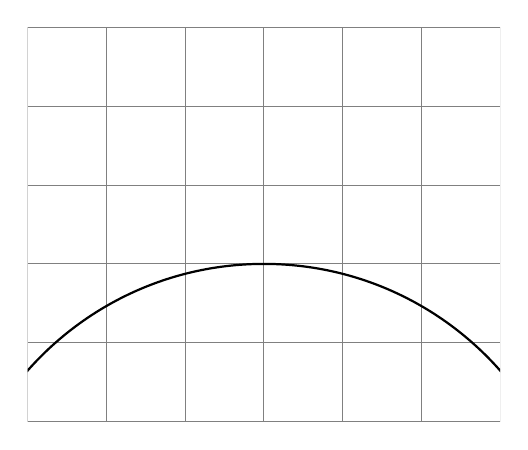
\begin{tikzpicture}
    \path[use as bounding box,clip] (-3,-2) rectangle (3,3);
    \draw[thin,gray] (-5,-5) grid (5,5);
    \coordinate (P) at (0,0);
    \coordinate (L) at (-1,2);
    \coordinate (E) at (2,1);
    \draw[thick] (0,-4) circle (4);
    \point[/point/label=P,/point/position=(P)]
    \point[/point/label=L,/point/position=(L)]
    \point[/point/label=E,/point/position=(E)]
  \end{tikzpicture}
\end{center}
\begin{center}
  \begin{tabular}{lcccc}
    & \textbf{r} & \textbf{g} & \textbf{b} \\
    \toprule
    light source & 1 & 1 & 0 \\
    ambient & 0.2 & 0.2 & 0.2 \\
    diffuse & 0.8 & 0.0 & 0.9 \\
    specular & 0.5 & 0.5 & 0.5 & e = 10
  \end{tabular}
\end{center}
\end{Exercise}


\begin{Exercise}
A sphere is centred at $C(3, 0, 0)$ and has radius $2$.
A ray of light starts at $P(2,2,2)$ and is directed straight towards
the sphere's centre. It hits the sphere at some position $H$.
The ray bounces off the sphere in a mirror-like way and proceeds to hit the YZ-plane at some point $Q$.
\begin{itemize}
  \item What are $H$'s coordinates?
  \item What is the reflected ray's direction?
  \item What are $Q$'s coordinates?
\end{itemize}
\end{Exercise}

\begin{Exercise}
A light ray traverses a piece of glass.
\begin{center}
  \begin{tikzpicture}
    \draw[thick] (0,0) -- ++(0,2);
    \draw[thick] (5,0) -- ++(0,2);
    \draw[light] (-1,2) -- (0,1.5) -- (5,0.5) -- (6,0);

    \draw[|-|,thin] (0,-.5) -- ++(5,0) node[below,midway] {5};
    \draw[dashed,thin] (0,1.5) -- (6,1.5);
    \draw[dashed,thin] (5,0.5) -- (6,0.5);
    \draw[|-|,thin] (6.5,0.5) -- (6.5,1.5) node[right,midway] {x};

    \node at (-2,0) {air};
    \node at (2.5,0) {glass};
    \node at (7,0) {air};
  \end{tikzpicture}
\end{center}
\end{Exercise}
The direction of the light is $(2,-1)$, the thickness of the glass is 5. What is vertical distance travelled by the light ray, represented by $x$?

\section{Ray Tracer}
\begin{Exercise}
Give the SDL file that produces this result:
\begin{center}
  \includegraphics[width=.5\linewidth]{scene.png}
\end{center}
The camera is located at $(0,0,-5)$, looks at $(0,0,0)$ and has up-vector $(0,1,0)$.
The sphere in the middle has radius 1; the lower sphere is twice as big.
Make sure not to forget about the following details:
\begin{itemize}
  \item The lights
  \item The material's properties (these do not have to be 100\% correct)
  \item The exact transformations.
\end{itemize}
\end{Exercise}

\section{Extensions}
\begin{Exercise}
Currently, our ray tracer allows us to specify only one colour to each shape:
a shape is either completely red, or blue, or white, or \dots
Say we want to achieve the following:
\begin{center}
  \includegraphics[width=.5\linewidth]{3d-textures.png}
\end{center}
What changes would you make to the ray tracer?
\end{Exercise}

\begin{Exercise}
Our shapes are perfectly smooth. It might come in handy to give them a rougher surface.
Take for example the bumpy sphere shown below.
\begin{center}
  \includegraphics[width=.5\linewidth]{bumpmapping.png}
\end{center}
What changes would you make to the ray tracer?
\end{Exercise}

\begin{Exercise}
Our ray tracer understands unions of objects, i.e. it is possible to create
a new shape by grouping two shapes together. There are other operations
like this, which yield more interesting results. Below you can see the result
of \emph{intersecting} two spheres to produce a lens.
\begin{center}
  \includegraphics[width=.5\linewidth]{csg.png}
\end{center}
What changes would you make to support intersection?
\end{Exercise}


%%% Local Variables:
%%% mode: latex
%%% TeX-master: "reference"
%%% End:
